% !TEX root = ../main.tex

Since the previous models inherently do not work in our setting, a natural definition would be to give the adversary control over 
scheduling on channels from only his corrupted parties. However, we will show that any reasonable 
model in which the adversary has the ability to delay messages for an 
unbounded 
amount of time allows him to learn something about the topology of the graph.
In essence, a very long delay from a party behaves almost like an abort, and 
an 
adversary can exploit this much like a fail-stop adversary in the 
impossibility 
result of \cite{MOR15}. We formally prove this in a very weak 
adversarial model.

First, note that if we have bounded delays, we can always use a synchronous protocol, starting the next round after waiting the maximum delay. So, in order for this model to be interesting, we must assume the adversary has unbounded delays.
In order to be as general as possible, we prove this with the weakest model we can while still giving the adversary some control over its delays: the adversary can only add delay to messages leaving corrupt nodes.

Our proof will follow the structure of \cite{MOR15}, using a similar game-based definition and even using the same adversarially-chosen graphs (see figure \ref{fig:imp}). Our game is straightforward. The adversary gives the challenger two graphs and a set of corrupt nodes so that the corrupt neighborhoods are identical when there is no adversarially added delay. The challenger then chooses one of those graphs at random, runs the protocol, and gives the views of all corrupt nodes to the adversary. The adversary wins if she can tell which graph was used. In \cite{MOR15}, the adversary would choose a round to failstop one of its corrupt parties. In our model, the adversary will instead choose a time (clock-tick) to add what we call a long-delay (which is just a very long delay on sending that and all subsequent messages). The adversary will be able to detect the delay based on when the protocol ends: if the delay was early in the protocol, the protocol takes longer to finish for all parties, and if it was late, the protocol will still finish quickly for most parties.

This impossibility result translates to an impossibility in the simulation-based setting since a secure protocol for the simulation-based setting would imply a secure protocol for the game-based setting.

Since delays cannot depend on the adversary without leaking topology, delays 
are an inherent property of the given network, much like in real life. As 
stated before, we give each edge a delay distribution, and the delays of 
messages traveling along that edge are sampled from this distribution. This 
allows us to model real-life networks where the adversary cannot tamper with 
the network connections. For example, on the Internet, delays between two 
directly connected nodes depend on their distance and the reliability of their 
connection.

\begin{figure}
	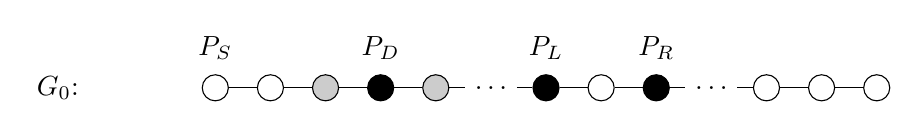
\begin{tikzpicture}[
	edge/.style={-}
	]
	\node at (-2,0) {$G_0$:};
	
	\def\dist{0.7}
	\node[circle,draw] (v1) at (0,0) {}; \node at (0,0.5) {$P_S$}; %{$P_1$}; 
	\node[circle,draw] (v2) at (\dist,0) {};
	\node[circle,draw,fill=black!20] (v3) at (2*\dist,0) {}; \node at (2*\dist,0.5) {};%{$P_3$}; 
	\node[circle,draw,fill=black] (v4) at (3*\dist,0) {}; \node at (3*\dist,0.5) {$P_D$};%{$P_4$}; 
	\node[circle,draw,fill=black!20] (v5) at (4*\dist,0) {}; \node at (4*\dist,0.5) {};%{$P_5$}; 
	\node[] (v6) at (5*\dist,0) {$\dots$};
	\node[circle,draw,fill=black] (v7) at (6*\dist,0) {}; \node at (6*\dist,0.5) {$P_L$};%{$P_{\frac{n}{2}-1}$}; 
	\node[circle,draw] (v8) at (7*\dist,0) {};
	\node[circle,draw,fill=black] (v9) at (8*\dist,0) {}; \node at (8*\dist,0.5) {$P_R$};%{$P_{\frac{n}{2}+1}$}; 
	\node[] (v10) at (9*\dist,0) {$\dots$};
	\node[circle,draw] (v11) at (10*\dist,0) {};
	\node[circle,draw] (v12) at (11*\dist,0) {};
	\node[circle,draw] (v13) at (12*\dist,0) {};
	
	\draw[edge] (v1) -- (v2) -- (v3) -- (v4) -- (v5) -- (v6) -- (v7) -- (v8) -- (v9)
	-- (v10) -- (v11) -- (v12) -- (v13);
	\end{tikzpicture}
	
	\medskip
	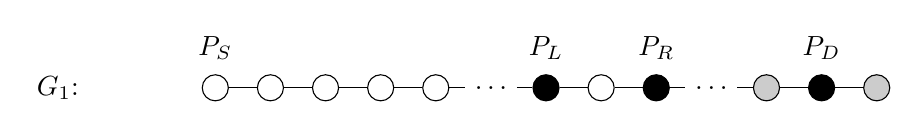
\begin{tikzpicture}[
	edge/.style={-}
	]
	\def\dist{0.7}
	\node at (-2,0) {$G_1$:};
	
	\node[circle,draw] (v1) at (0,0) {}; \node at (0,0.5) {$P_S$}; %{$P_1$}; 
	\node[circle,draw] (v2) at (\dist,0) {};
	\node[circle,draw] (v3) at (2*\dist,0) {}; 
	\node[circle,draw] (v4) at (3*\dist,0) {}; 
	\node[circle,draw] (v5) at (4*\dist,0) {}; 
	\node[] (v6) at (5*\dist,0) {$\dots$};
	\node[circle,draw,fill=black] (v7) at (6*\dist,0) {}; \node at (6*\dist,0.5) {$P_L$};%{$P_{\frac{n}{2}-1}$}; 
	\node[circle,draw] (v8) at (7*\dist,0) {};
	\node[circle,draw, fill=black] (v9) at (8*\dist,0) {}; \node at (8*\dist,0.5) {$P_R$};%{$P_{\frac{n}{2}+1}$}; 
	\node[] (v10) at (9*\dist,0) {$\dots$};
	\node[circle,draw,fill=black!20] (v11) at (10*\dist,0) {}; \node at (10*\dist,0.5) {};%{$P_3$}; 
	\node[circle,draw,fill=black] (v12) at (11*\dist,0) {}; \node at (11*\dist,0.5) {$P_D$}; %{$P_4$}; 
	\node[circle,draw,fill=black!20] (v13) at (12*\dist,0) {}; \node at (12*\dist,0.5) {};%{$P_5$};
	
	\draw[edge] (v1) -- (v2) -- (v3) -- (v4) -- (v5) -- (v6) -- (v7) -- (v8) -- (v9)
	-- (v10) -- (v11) -- (v12) -- (v13);
	\end{tikzpicture}
	\caption{Graphs used to prove the impossibility of THC with adversarial delays. 
		$P_S$ is the sender.
		The corrupted parties (black dots) are: $P_L$ and $P_R$ (they delay messages), and the detective $P_D$. The adversary determines whether $P_D$ (and its two neighbors) are on the left or on the right.}
	\label{fig:imp}
\end{figure}



\subsubsection{Adversarially-Controlled Delay Indistinguishability-based Security Definition}
Before proving the impossibility result, we first formally define our model. This model is as weak as possible while still assuming delays are somewhat controlled by the adversary. We will assume a minimum delay along edges: it takes at least one clock-tick for a message to get from one party to another.

\paragraph{Time and Clocks.}
Many asynchronous or semi-synchronous settings require defining a clock (or clocks) for the parties to use. This is to model the time passing in the real-world so that parties can adapt when messages are not delivered in time, etc. For this impossibility result, however, we only need the adversary to be able to keep track of the time passed. So, when the protocol starts, the adversary only needs to count `ticks,' the smallest unit of time that, say, a global clock would use. This way, it does not matter what other clock functionalities are present in the protocol's model, the adversary ignores it to mount its attack.

For notation, the adversary will mark the time passed by $\tau$.

\paragraph{Delay Algorithms}
In order to give the adversary as little power as possible, we define a public (and arbitrary) randomized algorithm that outputs the delays for a graph for protocol $\Pi$. Both the adversary and challenger have access to this algorithm and can sample from it.

\newcommand{\delayAlg}{\mathsf{DelayAlgorithm}}
\begin{definition}
	A \emph{indistinguishability-delay algorithm (IDA)} for a protocol $\Pi$, $\mathsf{Delay}$\-$\mathsf{Algorithm}_{\Pi}$, is a probabilistic polynomial-time algorithm that takes as input an arbitrary graph outputs unbounded polynomial delays for every time $\tau$ and every edge in the graph. Explicitly, for any graph $G = (V, E)$, $\delayAlg(G)$ outputs $\cT$ such that for every edge $(i,j) \in E_b$ and time $\tau$, $\cT((i,j), \tau) = d_{(i,j), \tau}$ is a delay that is at least one.
\end{definition}

\paragraph{The Indistinguishability Game}
This indistinguishability definition is a game between an adversary $\cA$ and challenger $\cC$ adapted from \cite{MOR15}. Let $\delayAlg$ be an IDA as defined above.
\begin{itemize}
	\item Setup: Let $\cG$ be a class of graphs and $\Pi$ a topology-hiding broadcast protocol that works on any of the networks described by $\cG$ according to our adversarial delay model, and let $\delayAlg$ be a public, fixed IDA algorithm. Without loss of generality, let $\party_1$ have input $x \in \{0,1\}$, the broadcast bit.
	\item $\cA$ chooses two graphs $G_0 = (V_0, E_0)$ and $G_1 = (V_1, E_1)$ from $\cG$ and then a subset $\CS$ of the parties to corrupt. $\CS$ must look locally the same in both $G_0$ and $G_1$. Formally, $\CS \subset V_0 \cap V_1$ and $\nbhi{0}{\CS} = \nbhi{1}{\CS}$. If this doesn't hold, $\cC$ wins automatically.\\
	$\cA$ then generates $\cT_{\CS}$, a function defining delays for every edge at every time-step controlled by the adversary. That is, $\cT_{\CS}((i,j), \tau) = d_{(i,j),\tau}$, and if $\party_i \in \CS$, then every message sent from $\party_i$ to $\party_j$ at time $\tau$ is delayed by an extra $d_{(i,j), \tau}$.\\
	$\cA$ sends $G_0, G_1, \CS,$ and $\cT_{\CS}$ to $\cC$.
	
	\item $\cC$ chooses a random $b \in \{0,1\}$ and executes $\Pi$ in $G_b$ with delays according to $\delayAlg(G_b) = \cT$ for all messages sent from honest parties. For messages sent from corrupt parties, delay is determined by the time and parties as follows: for time $\tau$ a message sent from party $\party_i \in \CS$ to $\party_j$ has delay $\cT((i,j), \tau) + \cT_{\CS}((i,j), \tau)$ in reaching $\party_j$. $\cA$ receives the view of all parties in $\CS$ during the execution.
	
	\item $\cA$ then outputs $b' \in \{0,1\}$ and wins if $b' = b$ and loses otherwise.
\end{itemize}

Notice that in this model, the adversary statically and passively corrupts any set of parties, and statically determines what delays to add to the protocol.

\begin{definition}
	A protocol $\Pi$ is \emph{indistinguishable under chosen delay attack (IND-CDA)} over a class of graphs $\cG$ if for any PPT adversary $\cA$, there exists an IDA $\delayAlg$ such that
	\[ \Pr[\cA \mbox{ wins}]  \leq \frac 1 2 + \negl(n). \]
\end{definition}

\subsubsection{Proof that Adversarially-Controlled Delays Leak Topology}
First, we will define what we mean when we say a protocol is `weakly' realized in the adversarial delay model. Intuitively, it is just that the protocol outputs the correct bit to all parties if there is no adversarial delay.

\begin{definition}
	A protocol $\Pi$ \emph{weakly realizes the broadcast functionality} if $\Pi$ is such that when all parties execute honestly with delays determined by any IDA, all parties get the broadcast bit within polynomial time (with all but negligible probability).
\end{definition}


\begin{theorem}\label{thm:impossibility}
	There does not exist an IND-CDA secure protocol $\Pi$ that weakly realizes the broadcast functionality of any class of graphs $\cG$ that contains line graphs.
\end{theorem}

Throughout the proof and associated claim, we refer to a specific pair of graphs that the adversary has chosen to distinguish between, winning the IND-CDA game. Both graphs will be a line of $n$ vertices: $G = (V,E)$ where $E = \{(\party_i, \party_{i+1})\}_{i=1,\ldots,n-1}$. We will let $\Pi$ be a protocol executed on $G$ that weakly realizes broadcast when $P_1$ is the broadcaster, see Figure \ref{fig:imp}.

Our adversary in this model will either add no delay, or will add a very long polynomial delay to every message sent after some time $\tau$.

Notice that $\cA$ is given access to $\delayAlg$ at the start of the protocol. One can sample from $\delayAlg$ using $G_0$, $G_1$, and $\CS$ to get an upper bound $T$ on the time it takes $\Pi$ to terminate with all but negligible probability. Since $\Pi$ weakly realizes broadcast, $T$ is polynomial. So, $\cA$ has access to this upper bound $T$.


\paragraph{Long-delays.} Let a long-delay be a delay that lasts for $T$ clock-ticks. Consider an adversary that will only add long-delays to a protocol, and once an adversary has long-delayed a message, he must continue to long-delay messages along that edge until the end of the protocol. That is, once the adverary decides to delay along some edge, all subsequent messages along that edge cannot arrive for at least $T$ clock-ticks.

\begin{claim}
	Consider any party $\party_v$ whose neighbors do not add any extra delay as described by the long-delay paragraph above. As in \cite{MOR15}, let $H_{v,b}$ be the event that $\party_v$ outputs the broadcast bit by time $T$ ($\party_v$ may still be running the protocol by time $T$ or terminate by guessing a bit by $T$). 
	Let $E_\tau$ be the event that the first long-delay is at time $\tau$. Then either $\Pi$ is not IND-CDA secure, or there exists a bit $b$ such that 
	\[ \lvert \Pr \left[ H_{v,b} | E_{T-1} \right] - \Pr \left[ H_{v,b} | E_{0} \right] \rvert \geq \frac 1 2 - \negl(n).\]
\end{claim}
\begin{proof}
	If some $\party_i$ long-delays at time $0$, then the first message it sends is at time $T$, and so the graph is disconnected until time $T$. This makes it impossible for parties separated from $\party_1$ to learn about the output bit by time $T$. So, by that time, these parties must either guess an output bit (and be right with probability at most 1/2) or output nothing and keep running the protocol (which is still not $H_{v,b}$). If $\Pi$ is IND-CDA secure, then all honest parties must have the same probability of outputting the output bit by time $T$, and so there exists a $b$ such that $\Pr[H_{v,b} | E_0] \leq \frac 1 2 - \negl(n)$ for all honest parties $\party_v$.
	
	However, if $\party_i$ long-delays at time $T-1$, then the only parties possibly affected by $\party_i$ are $\party_{i-1}$ and $\party_{i+1}$; all other parties will get the output by time $T$ and the information that $\party_i$ delayed cannot reach them (recall we assumed a minimum delay of at least one clock-tick in the $\delayAlg$). So, $\Pr[H_{v,b} | E_0] = \Pr[H_{v,b} | \mbox{no extra delays}] = 1 - \negl(n)$ for all honest parties without a delaying neighbor by the definition of weakly realizing broadcast.
	
	The claim follows: $\lvert \Pr \left[ H_{v,b} | E_{T-1} \right] - \Pr \left[ H_{v,b} | E_{0} \right] \rvert \geq \lvert \frac 1 2 - \negl(n) - 1 
	\rvert \geq \frac 1 2 - \negl(n)$.
	\qed
\end{proof}

\begin{proof}[Theorem \ref{thm:impossibility}]
	This just follows from the previous claim. A simple hybrid argument shows that there exists a pair $(\tau^*, b) \in \{0,\ldots, T-1\} \times \{0,1\}$ such that 
	\[ \lvert \Pr \left[H_{v,b} | E_{\tau^*} \right] - \Pr \left[ H_{v,b} | E_{\tau^* + 1} \right] \rvert \geq \frac 1 {2T} - \negl(n) \]
	for all $P_v$ who do not have a neighbor delaying. Since $T$ is polynomial, this is a non-negligible value. Without loss of generality, assume $\Pr[ H_{v,b} | E_{\tau^*}] > \Pr[H_{v,b} | E_{\tau^* + 1}]$. Leveraging this difference, we will construct an adversary $\cA$ that can win the IND-CDA game with non-negligible probability.
	
	$\cA$ chooses two graphs $G_0$ and $G_1$. $G = G_0$ and $G_1$ is $G$ except parties 3, 4, and 5 are exchanged with parties $n-2$, $n-1$, and $n$ respectively. $\cA$ corrupts the source part $\party_S := \party_1$, a left party $\party_L := \party_{n/2-1}$, a right party $\party_R := \party_{n/2 + 1}$, and the detective party $\party_D := \party_4$. See figure \ref{fig:imp} for how this looks. The goal of $\cA$ will be to determine if $\party_D$ is to the left or right side of the network (close to the broadcaster or far).
	
	$\cA$ computes the upper bound $T$ using $\delayAlg$ and randomly guesses $(\tau^*, b)$ that satisfy the inequality above. At time $\tau$, $\cA$ initiates a long-delay at party $\party_L$, and at time $\tau+1$, $\cA$ initiates a long-delay at party $\party_R$. So, $\cA$ gives the challenger $\cT_{\CS}$ where $\cT_{\CS}((i,j), t) = 0$ for $t < \tau^*$, and for $t \geq \tau^*$: $\cT_{\CS}((L, n/2), t) = \cT_{\CS}((L, n/2-2), t) T$ and $\cT_{\CS}((R, n/2), t+1) = \cT_{\CS}((R, n/2 + 2), t+1) = T$.
	
	Notice that news of $P_L$'s delay at time $\tau^*$ cannot reach $P_R$ or any other party on the right side of the graph by time $T$. Also note that the time $\cA$ gets output for each of its corrupt parties is noted in the trasncript.
	
	If $\cC$ chooses $G_0$, then $\party_D$ is on the left side of the graph and has probability $\Pr[H_{D, b} | E_{\tau^*}]$ of having the output bit by time $T$ because its view is consistent with $\party_L$ delaying at time $\tau^*$.
	If $\cC$ chooses $G_1$, then $\party_D$ is on the right side of the graph, and has a view consistent with the first long delay happening at time $\tau^*+1$ and therefore has $\Pr[H_{D,b} | E_{\tau^*}]$ of having the output bit by time $T$.
	Because there is a noticeable difference in these probabilities, $\cA$ can distinguish between these two cases with $\frac 1 2$ plus some non-negligible probability.
\end{proof}

\paragraph{Consequences of this lower bound.}
We note that this is just one model where we prove it is impossible for the adversary to control delays. However, we restrict the adversary a great deal, to the point of saying that regardless of what the natural network delays are, the adversary can learn something about the topology of the graph. The lower bound proved in this model seems to rule out any possible model (simulation or game-based) where the adversary has power over delays.



